\documentclass[12pt,a4paper]{report}
% Packages for enhanced functionality
\usepackage[utf8]{inputenc}
\usepackage[T1]{fontenc}
\usepackage{graphicx} % For including images
\usepackage{geometry} % For page layout
\usepackage{hyperref} % For clickable links and references
\usepackage{fancyhdr} % For custom headers and footers
\usepackage{titlesec} % For section title formatting
\usepackage{float}
\usepackage{circuitikz}
\usepackage{caption}
\usepackage{siunitx}
\usepackage{amsmath}
\usepackage{subcaption}
\usepackage{booktabs}
\newcommand{\vecb}[1]{\mathbf{#1}}
\newcommand{\brak}[1]{\ensuremath{\left(#1\right)}}
\newcommand{\cbrak}[1]{\ensuremath{\left\{#1\right\}}}
\newcommand{\abs}[1]{\left\vert#1\right\vert}
\newcommand{\norm}[1]{\left\lVert#1\right\rVert}
\providecommand{\sbrak}[1]{\ensuremath{{}\left[#1\right]}}
\providecommand{\lsbrak}[1]{\ensuremath{{}\left[#1\right.}}
\providecommand{\rsbrak}[1]{\ensuremath{{}\left.#1\right]}}
\providecommand{\brak}[1]{\ensuremath{\left(#1\right)}}
\providecommand{\lbrak}[1]{\ensuremath{\left(#1\right.}}
\providecommand{\rbrak}[1]{\ensuremath{\left.#1\right)}}
\providecommand{\cbrak}[1]{\ensuremath{\left\{#1\right\}}}
\providecommand{\lcbrak}[1]{\ensuremath{\left\{#1\right.}}
\providecommand{\rcbrak}[1]{\ensuremath{\left.#1\right\}}}
\hypersetup{
    colorlinks=true,  % Enable colored text links
    linkcolor=orange,    % Internal links (sections, table of contents, etc.)
    urlcolor=orange,     % External URLs
    citecolor=orange,    % Citations
    pdfborder={0 0 0} % Remove ugly default borders
}
\begin{document}
\title{\textbf{EE1060 Quiz 6}\\
\LARGE{\textbf{ }}

\author{ Arjun Pavanje(EE24BTECH11005)\\M.B.S.Aravind (EE24BTECH11038)\\Shiny Diavajna.P (EE24BTECH11058)\\Homa Harshitha.V (EE24BTECH11062)\\Shivam Shilvant (EE24BTECH11057)\\Pranay Kumar.B (EE24BTECH11011)}

\begin{center}
\end{center}
\vspace{30pt}
\begin{figure}[ht]
	\centering
	
\includegraphics[width = 100pt]{logo.png}\\
\end{figure}
\begin{center}
	Bachelor of Technology\\
	\vspace{10pt}
	Department of Electrical Engineering\\
\end{center}
}
\maketitle

% Title page settings
%\title{
%    \vspace{2in}
%    \Huge{\textbf{}} \\
%    \Large{} \\
%    \vspace{1in}
%    \vspace{1in}
%    \Large{Arjun Pavanje(EE24BTECH11005)\\M.B.S.Aravind (EE24BTECH11038)\\Shiny Diavajna.P (EE24BTECH11058)\\Homa Harshitha.V (EE24BTECH11062)\\Shivam Shilvant (EE24BTECH11057)\\Pranay Kumar.B (EE24BTECH11011)}\\
%    \Large{Date: \today}
%}
%\author{}
%\date{}
%% Section title formatting
%\titleformat{\chapter}[hang]{\Huge\bfseries}{\thechapter.}{20pt}{}
%\titleformat{\section}[hang]{\Large\bfseries}{\thesection}{12pt}{}
%\titleformat{\subsection}[hang]{\large\bfseries}{\thesubsection}{10pt}{}
%\begin{document}
%% Title page
%\maketitle

% Table of Contents
\tableofcontents
\chapter{Introduction}
    The goal of this report is to study the convolution of a signal with a rectangular kernel, analyze how shifting and modifying the kernel affects the output and understand the system’s behavior under various conditions.\\
    The rectangular kernel is defined as :\\\\
    \[h(t) = \begin{cases}
1, & \text{for } -T \leq t \leq T \\
0, & \text{otherwise}
\end{cases}
\]

\begin{center}
\begin{tikzpicture}[scale=1]
  % Axes
  \draw[->] (-3.5,0) -- (3.5,0) node[right] {\( t \)};
  \draw[->] (0,-0.5) -- (0,2.5) node[above] {\( h(t) \)};

  % Rectangular pulse
  \draw[thick] (-2,0) -- (-2,2) -- (2,2) -- (2,0);

  % Dotted lines and labels for T
  \draw[dashed] (-2,0) -- (-2,-0.2) node[below] {\( -T \)};
  \draw[dashed] (2,0) -- (2,-0.2) node[below] {\( T \)};
  \node at (-2.2,2) {1};
\end{tikzpicture}
 


\end{center}
\section{Convolution :}
\section*{Overview}

Convolution is a powerful mathematical operation widely used in engineering, physics, and signal processing. Closely tied to Fourier transforms, convolution helps describe how systems respond to inputs over time or space.

\section*{Definition}

Mathematically, the convolution of two functions \( f(x) \) and \( g(x) \) is defined as:

\[
(f * g)(t) = \int_{-\infty}^{\infty} f(\tau) \cdot g(t - \tau) \, d\tau
\]

Alternatively, it can be written by switching the roles of the functions (convolution is commutative),

\[
(f * g)(\tau) = \int_{-\infty}^{\infty} g(\tau) \cdot f(t - \tau) \, d\tau
\]

This operation effectively combines two functions by sliding one across the other, multiplying pointwise values, and integrating the result.
\section*{Intuitive Understanding}

We can think of convolution as a weighted averaging process. We can imagine that one function represents a signal, and the other acts as a filter or response function. As one function slides over the other, their overlap determines the value of the output. The integral collects these weighted overlaps across the domain.

\section*{Convolution and the Fourier Transform}

One of the most useful aspects of convolution is its relationship with Fourier transforms. The \textbf{Convolution Theorem} states:

\begin{itemize}
    \item The Fourier transform of a convolution is the product of the individual Fourier transforms:
    \[
    \mathcal{F}\{f * g\} = \mathcal{F}\{f\} \cdot \mathcal{F}\{g\}
    \]
    
    \item Conversely, the Fourier transform of a product is the convolution of the transforms:
    \[
    \mathcal{F}\{f \cdot g\} = \mathcal{F}\{f\} * \mathcal{F}\{g\}
    \]
\end{itemize}

This relationship allows easier computation of convolutions in the frequency domain.
\section*{Convolution with a Rectangular Kernel}

The output of an LTI system with impulse response $h(t)$ and input $f(t)$ is given by the convolution integral
\[
y(t) = (f*h)(t) = \int_{-\infty}^{\infty} f(\tau)\, h(t-\tau)\, d\tau,
\]
which ``slides'' one function over another and integrates their product. In our case, $h(t) = 1$ for $-T \leq t \leq T$ and $0$ otherwise. Thus, $h(t-\tau) = 1$ exactly when $\tau \in [t-T,\;t+T]$. The convolution becomes
\[
y(t) = \int_{max(0,t-T)}^{t+T} f(\tau)\, d\tau.
\]
In short, the output is the \textbf{sliding integral} (or running sum) of $f$ over the interval of length $2T$.


\section{Step Input ($f(t) = u(t)$)}
Convolving a unit step with the symmetric box yields a \textbf{ramp} that saturates. Specifically:
\begin{itemize}
    \item y(t)=(x * h)(t) = $\int_{max(0,t -T)}^{T+t} 1 \, d\tau$\\
    \item For $t < -T$, the interval $[t-T, t+T]$ lies entirely before $0$, so $y(t) = 0$.
    \item For $-T \leq t < T$, the box partially overlaps the step:
    \[
    y(t) = \int_{0}^{t+T} 1\, d\tau = t + T.
    \]
    Thus, $y(t)$ rises linearly from $0$ (at $t = -T$) up to $2T$ (at $t = T$).
    \item For $t \geq T$, the box fully covers the step:
    \[
    y(t) = \int_{t-T}^{t+T} 1\, d\tau = 2T.
    \]
\end{itemize}
Thus, $y(t)$ is triangular-shaped: it increases from $0$ to $2T$ over $[-T,T]$ and then stays constant.
\begin{figure}[H]
   \centering
   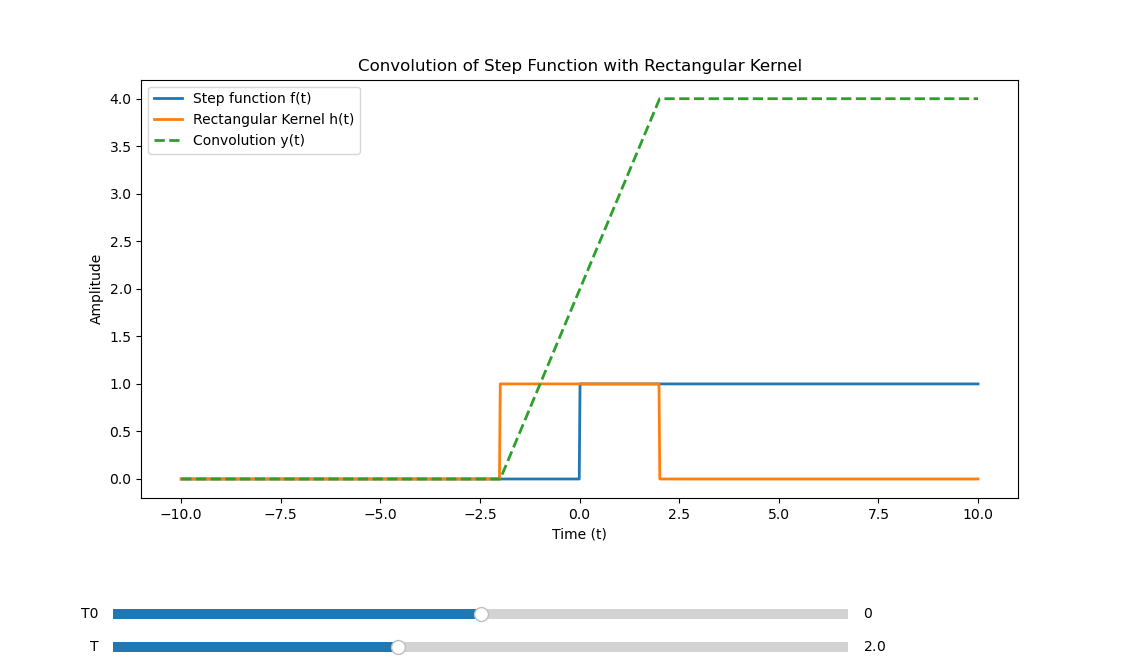
\includegraphics[width=1\textwidth, height=0.5\textheight]{figs/step_con.png}
\end{figure}

\section{Polynomial input}

Let the polynomial be given by:
\[
f(t) = a_n t^n + a_{n-1} t^{n-1} + \cdots + a_1 t + a_0
\]
The convolution simplifies to:

\[
y(t) = \int_{t-T}^{t+T} f(\tau) \, d\tau
\]

Substituting \( f(\tau) = a_n \tau^n + a_{n-1} \tau^{n-1} + \cdots + a_1 \tau + a_0 \), we get:

\[
y(t) = \int_{t-T}^{t+T} \left( a_n \tau^n + a_{n-1} \tau^{n-1} + \cdots + a_1 \tau + a_0 \right) \, d\tau
\]
For each term in the polynomial, we compute the integral.
For the \( \tau^n \) term:

\[
\int_{t-T}^{t+T} \tau^n \, d\tau = \left[ \frac{\tau^{n+1}}{n+1} \right]_{t-T}^{t+T} = \frac{(t+T)^{n+1} - (t-T)^{n+1}}{n+1}
\]
For the constant term :
\[
\int_{t-T}^{t+T} a_0 \, d\tau = a_0 \cdot \left[ \tau \right]_{t-T}^{t+T} = a_0 \cdot 2T
\]
Overall, the result is 
\begin{align*}
y_s(t)
&= \sum_{k=0}^n a_k \int_{t - T}^{t + T} \tau^k\,d\tau \\
&= \sum_{k=0}^n a_k \cdot \frac{(t + T)^{k + 1} - (t - T)^{k + 1}}{k + 1}.
\end{align*}

This is a polynomial of degree at most $n + 1$.\\
\begin{figure}[h!]
    \centering
    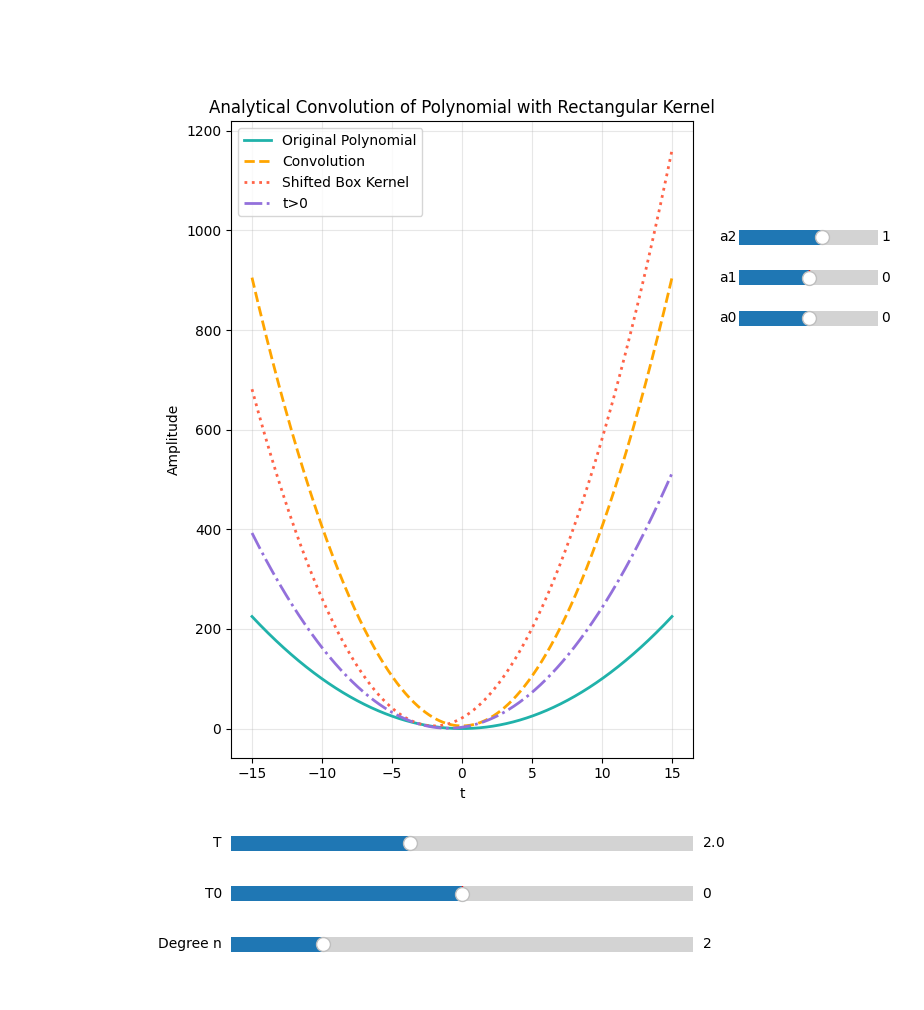
\includegraphics[width=0.8\linewidth]{figs/poly_conv.png}
    \label{fig:polynomial}
\end{figure}
This is convolution of polynomial $t^2$ with rectangle kernel taking $T=2$
\pagebreak
\section{Sinusoidal Input}
\begin{align*}
H\brak{\omega} = (f \ast h)\brak{t} &= \int_{-\infty}^\infty A\sin\brak{\omega \tau + \phi} \, h\brak{t - \tau} \, d\tau \\
&= A\int_{t-T}^{t+T} \sin\brak{\omega\tau + \phi}d\tau \\
&= \frac{A}{\omega}\sbrak{-\cos\brak{\omega\tau + \phi}}i_{t-T}^{t+T} \\
&= \frac{A}{\omega}\sbrak{\cos\brak{\omega (t-T)+  \phi} - \cos\brak{\omega (t+T) + \phi}} \\
&= \frac{2A}{\omega}\sin(\omega t + \phi)sin(\omega T)
\end{align*}
We observe, that if we convolve input signal $f\brak{t} = sin\brak{t}$ with box kernal, resultant signal is just scaled by a factor of $\frac{2}{\omega}\sin\brak{\omega T}$. Time period remains unchanged.
For low frequencies ($\omega \to 0$), $\sin(\omega T) \approx \omega T$, so $H(\omega) \approx 2T$. At higher frequencies, $|H(\omega)|$ falls off, and the rectangular window acts as a low-pass filter.
\begin{figure}[h!]
    \centering
    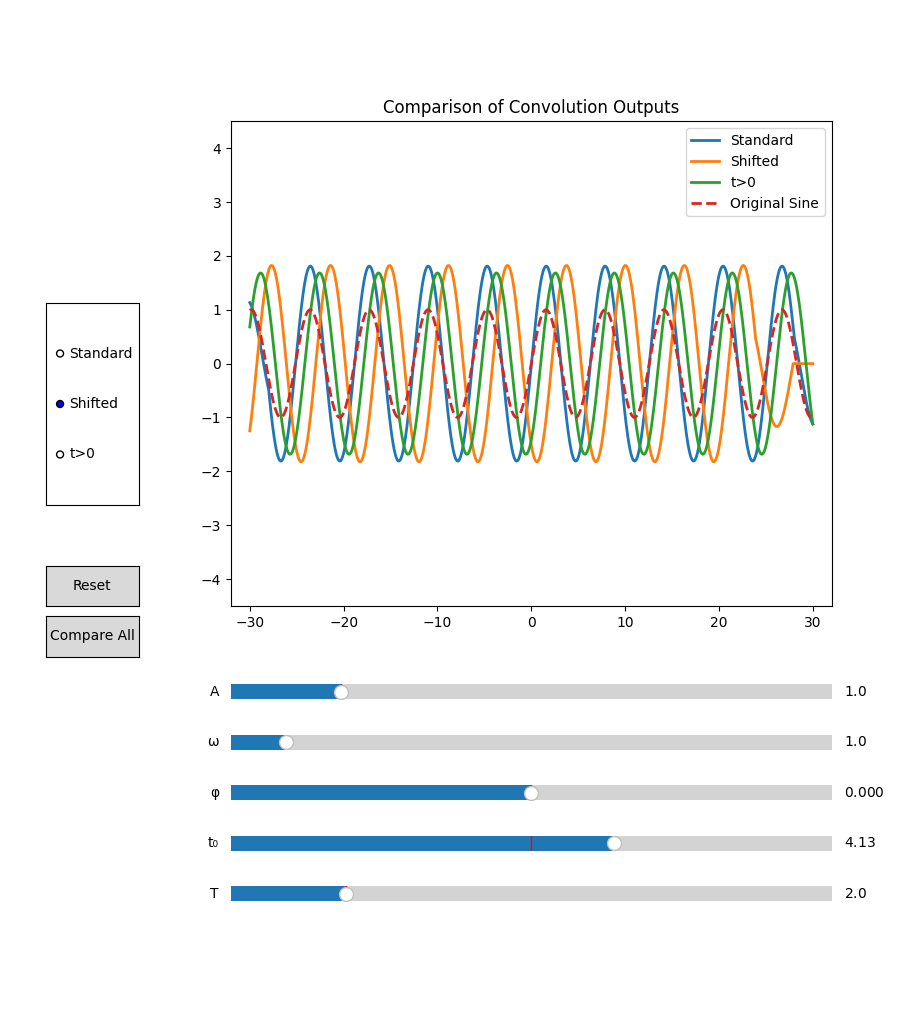
\includegraphics[width=0.6\linewidth]{figs/sine_conv.png}
    \label{fig:enter-label}
\end{figure}
\section{Impulse Input}
\begin{align*}
    \brak{f\ast h} &= \int_{-\infty}^{\infty} f\brak{\tau} h\brak{t-\tau}d\tau\\
    &= \int_{-\infty}^{\infty} \delta\brak{\tau} h\brak{t-\tau}d\tau\\ 
    &= h\brak{t}
\end{align*}
We observe that we get the rectangular kernel back as the output.
\begin{figure}[h!]
    \centering
    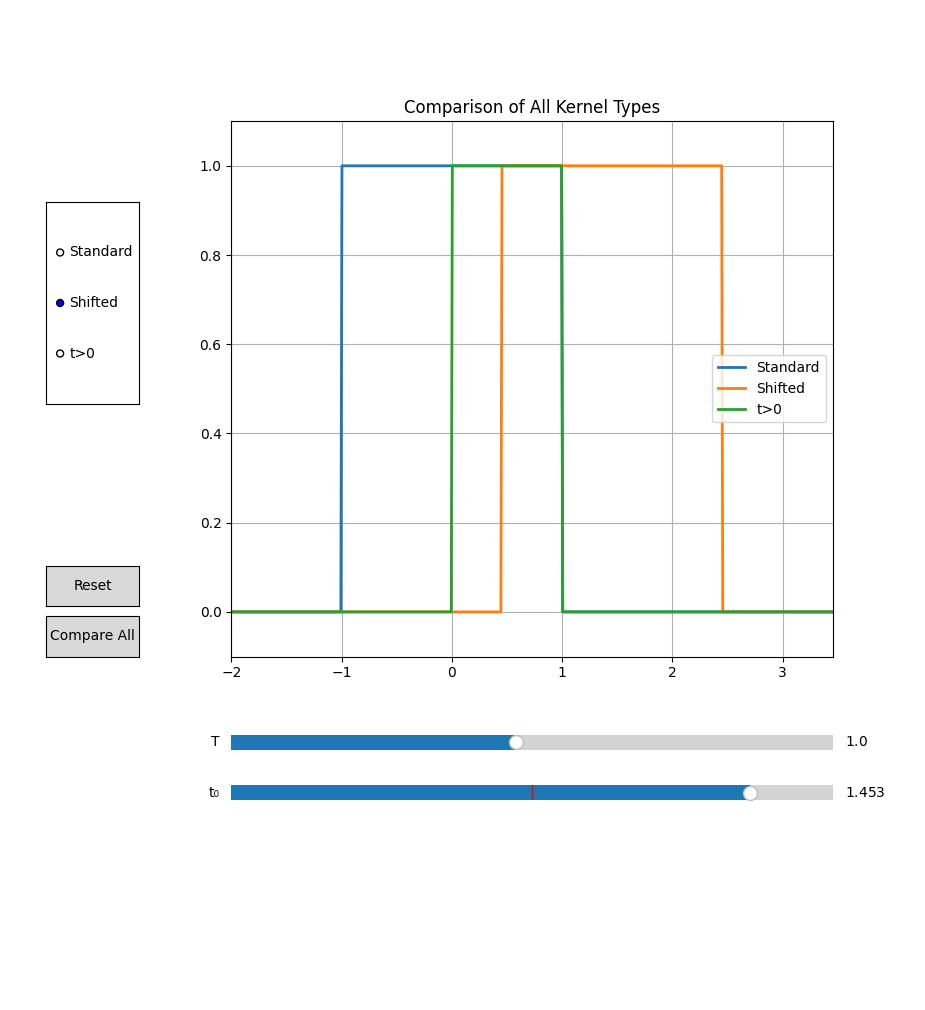
\includegraphics[width=0.7\linewidth]{figs/imp_conv.png}
    \label{fig:enter-label}
\end{figure}
\section{Expontial Function}
\begin{align*}
\brak{f \ast h} &= \int_{-\infty}^{\infty} e^{a\tau} h(t - \tau) d\tau \\
&= \int_{t-\tau_0-T}^{t-\tau_0+T} e^{a\tau} d\tau \\
&= \frac{1}{a} e^{a\tau} \Big|_{t-\tau_0-T}^{t-\tau_0+T} \\
&= \frac{e^{a(t-\tau_0+T)} - e^{a(t-\tau_0-T)}}{a} \\
&= \frac{2e^{a(t-\tau_0)}}{a} \sinh(aT)
\end{align*}
We get a  scaled hyperbolic sine function corresponding to input exponential wave as the result of convolution.
\begin{figure}[h!]
    \centering
    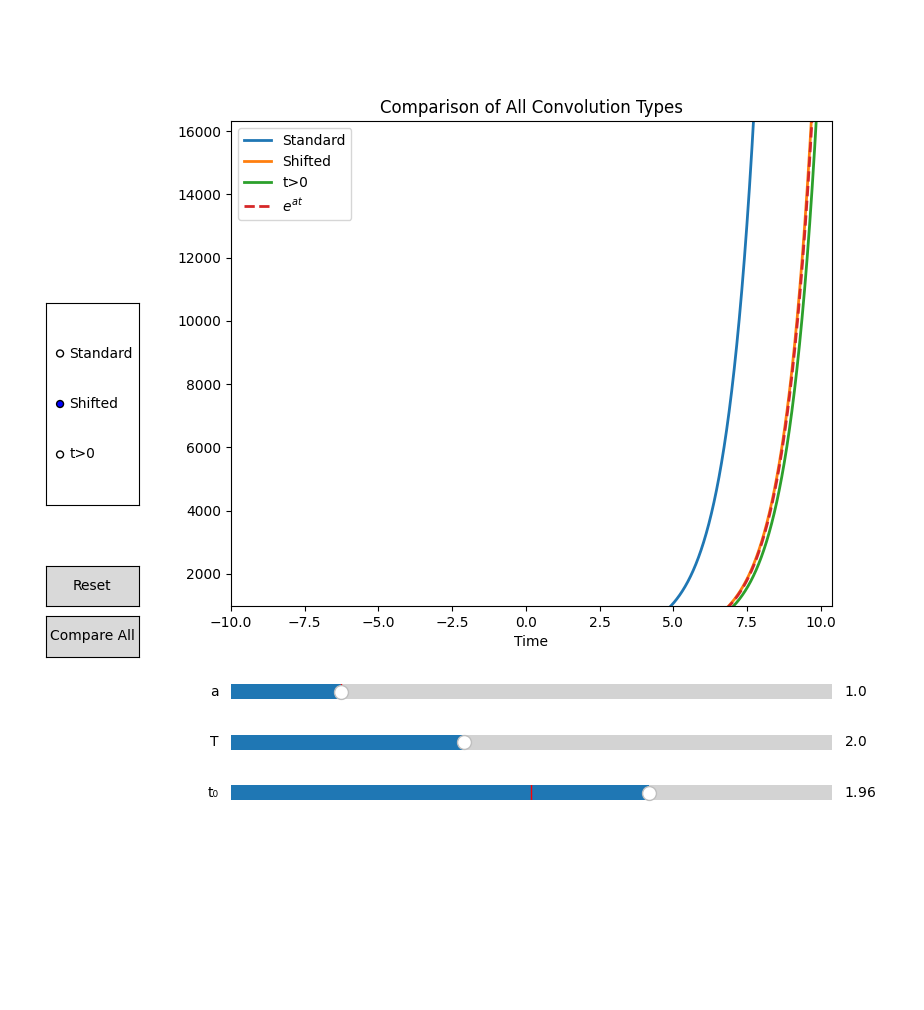
\includegraphics[width=0.7\linewidth]{figs/exp_conv.png}
    \label{fig:enter-label}
\end{figure}
\chapter{Behavior of the Convolution}
\section{Step input}
The result of the convolution is a piecewise-linear function with three distinct regions:

\begin{itemize}
    \item \textbf{Zero Region} ($t < T_0 - T$): No overlap between $u$ and $h$, hence $(u * h)(t) = 0$.
    \item \textbf{Linear Ramp} ($T_0 - T \leq t \leq T_0 + T$): Partial overlap; the output grows linearly:
    \[
    (u * h)(t) = t - (T_0 - T).
    \]
    \item \textbf{Plateau Region} ($t > T_0 + T$): Full overlap; the output is constant:
    \[
    (u * h)(t) = 2T.
    \]
\end{itemize}
\subsection{Specific Cases}

\begin{itemize}
    \item \textbf{$T=0$}: The kernel becomes a Dirac delta centered at $T_0$, and the convolution simply shifts the step function:
    \[
    (u * h)(t) = u(t - T_0).
    \]
    \item \textbf{Very small $T$}: The ramp is extremely narrow and steep; the output approximates a sharp step.
    \item \textbf{Very large $T$}: The ramp becomes extremely gradual and wide. Without normalization, the plateau height grows unbounded; with normalization, the rise becomes extremely slow.
    \item \textbf{$T_0=0$}: Symmetric case; ramp spans from $-T$ to $T$ around the origin.
\end{itemize}
\subsection{Graphical Interpretation}

The convolution measures the area of overlap between the step function and the sliding rectangular window.  
The output is:
\begin{itemize}
    \item $0$ when no overlap,
    \item proportional to the length of overlap during partial overlap (ramp region),
    \item maximal when full overlap (plateau region).
\end{itemize}
\section{Polynomial Input}

Let $f(t)$ be a polynomial of degree $n$ defined on the entire real line, and let $h(t)$ be a rectangular pulse of width $2T$ centered at $T_0$, i.e.,
\[
h(t) = \begin{cases}
1, & t \in [T_0 - T, T_0 + T] \\
0, & \text{otherwise}
\end{cases}
\]

The convolution $(f * h)(t)$ is given by:
\[
(f * h)(t) = \int_{-\infty}^{\infty} f(\tau) h(t - \tau)\,d\tau = \int_{t - (T_0 + T)}^{t - (T_0 - T)} f(\tau)\, d\tau
\]

\begin{itemize}
    \item \textbf{Smoothness:} Since $f$ is continuous and $h$ is piecewise continuous, the convolution is continuous and differentiable. The result is a polynomial of degree atmost $n+1$.
    
    \item \textbf{No Piecewise Behavior:} Because $f(t)$ has full (infinite) support, the convolution is defined for all $t \in \mathbf{R}$. The expression for $(f * h)(t)$ does not need to be split into regions, it’s a single, continuous polynomial.
    
    \item \textbf{Output Degree:} If $f(t)$ is degree-$n$, then $(f*h)(t)$ is degree-$(n+1)$ due to integration.
    
    \item \textbf{Moving Average:} The convolution acts as a moving average over a width $2T$, smoothing the input. The result can also be written as:
    $(f * h)(t) = \int_{-T}^{T} f(t - T_0 + \tau)\, d\tau$
    when re-centered around the kernel.
    
    \item \textbf{Specific Case $T_0 = 0$:} The kernel is symmetric about the origin. Then:
    \[
    (f * h)(t) = \int_{-T}^{T} f(t + \tau)\, d\tau
    \]
    which yields a symmetric smoothing operation with no phase shift.
\end{itemize}

\subsection{Graphical Interpretation}

\begin{itemize}
    \item The convolution at time $t$ computes the area under the polynomial $f(\tau)$ inside a window $[t - T, t + T]$.
    
    \item This results in a polynomial curve $(f * h)(t)$ that smooths the original function.
    
    \item The output is continuous and globally defined (infinite support), and it inherits smoothness and general shape from $f(t)$.
    
    \item As $T$ increases, the convolution becomes smoother and approximates a broader moving average.
\end{itemize}

\chapter{Causal (One-Sided) Rectangular Kernel}

Suppose $h(t) = 1$ for $0 \leq t \leq T$ and $0$ otherwise. Then,
\[
y(t) = \int_{max(0,t-T)}^{t} f(\tau)\, d\tau,
\]
for $t \geq 0$ (and $y(t) = 0$ for $t < 0$ if $f$ was zero for $t<0$).

\section{Step Input}
For $f(t) = u(t)$:
\[
y(t) =
\begin{cases}
t, & 0 \leq t < T,\\
T, & t \geq T.
\end{cases}
\]
Thus, $y(t)$ ramps up to $T$ and stays there.
\begin{itemize}
        \item For $t < 0$: output is $0$ (causal).
        \item For $0 \leq t < T$: output grows linearly (ramp).
        \item For $t \geq T$: output saturates to $T$ (plateau).
    \end{itemize}
\section{Polynomial input}
\begin{align*}
y_c(t) &= (f * h_c)(t) = \int_{-\infty}^\infty f(\tau) h_c(t - \tau)\,d\tau \\
&= \int_{t - T}^{t} f(\tau)\,d\tau \\
&= \sum_{k=0}^n a_k \int_{t - T}^{t} \tau^k\,d\tau \\
&= \sum_{k=0}^n a_k \cdot \frac{t^{k + 1} - (t - T)^{k + 1}}{k + 1}.
\end{align*}
\begin{itemize}
\item As $T \to 0$, the system approaches the identity:
    \[
    (f * h)(t) \to f(t).
    \]
    \item As $T$ increases, the smoothing window widens, and the high-frequency content in $f(t)$ gets suppressed more.
    \end{itemize}
\section{Sinusoidal Input}
Here, we take a modified $h\brak{t}$, which only considers the positive half of the function $t>0$.
\begin{align*}
    g\brak{t} = \begin{cases}
        1 & 0 \le t \le T\\
        0 & \text{Otherwise}
    \end{cases}
\end{align*}
\begin{align*}
(f \ast h)\brak{t} &= \int_{-\infty}^\infty A\sin\brak{\omega \tau + \phi} \, g\brak{t - \tau} \, d\tau \\
    &= \sbrak{-\frac{A}{\omega} \cos\brak{\omega \tau + \phi}}_{t-T}^t \\
    &= \frac{A}{\omega} \brak{\cos\brak{\omega t - \omega T + \phi} - \cos\brak{\omega t + \phi}}
\end{align*}
The Fourier transform of the one-sided box is
\[
H(\omega) = \int_{0}^{T} e^{-j\omega\tau}\, d\tau = \frac{1 - e^{-j\omega T}}{j\omega},
\]
which in magnitude behaves similarly to the symmetric box but introduces a phase shift. The output is a sinusoid scaled by $|H(\omega)|$ with a phase shift.
\section{Impulse Input}
Here, we take a modified $h\brak{t}$, which only considers the positive half of the function $t>0$.
\begin{align*}
    g\brak{t} = \begin{cases}
        1 & 0 \le t \le T\\
        0 & \text{Otherwise}
    \end{cases}
\end{align*}
\begin{align*}
    \brak{f\ast h} &= \int_{\infty}^{\infty} g\brak{\tau} g\brak{t-\tau}d\tau\\
    &= \int_{\infty}^{\infty} \delta\brak{\tau} g\brak{t-\tau}d\tau\\ 
    &= g\brak{t}
\end{align*}
This is basically the box kernel shifted to the right by $T$ and it's time period halved to $T$.
\section{Exponential Input}
Here, we take a modified $h\brak{t}$, which only considers the positive half of the function $t>0$.
\begin{align*}
    g\brak{t} = \begin{cases}
        1 & 0 \le t \le T\\
        0 & \text{Otherwise}
    \end{cases}
\end{align*}
\begin{align*}
\brak{f \ast h} &= \int_{t - T}^{t} e^{a\tau} \, d\tau \\
&= \left. \frac{1}{a} e^{a\tau} \right|_{t - T}^{t} \\
&= \frac{1}{a} \left( e^{at} - e^{a(t - T)} \right) \\
&= \frac{e^{at}}{a} \left(1 - e^{-aT}\right)
\end{align*}
\chapter{Time-Shifted Kernel}

If we shift the symmetric kernel by $\tau_0$, using $h_{\tau_0}(t) = h(t-\tau_0)$, then
\[
(f * h_{\tau_0})(t) = (f * h)(t - \tau_0).
\]
Thus, the output is simply a delayed version of the original output by $\tau_0$. In the frequency domain, this introduces a phase factor $e^{-j\omega \tau_0}$, representing a linear phase delay.

\section{Step input}

Changing the center $T_0$ affects:

\begin{itemize}
    \item \textbf{Horizontal Shift}: Increasing $T_0$ shifts the ramp and plateau to the right. Decreasing $T_0$ shifts them to the left.
    \item \textbf{Timing of Transition}: 
    \begin{itemize}
        \item Positive $T_0$ delays the onset of the ramp.
        \item Negative $T_0$ causes the ramp to begin earlier.
    \end{itemize}
\end{itemize}
\section{Polynomial input}

\begin{itemize}
    \item \textbf{Horizontal Shift}: Increasing $T_0$ shifts the smoothed polynomial to the right, while decreasing $T_0$ shifts it to the left.

    \item \textbf{Phase Relation}: 
    \begin{itemize}
        \item Positive $T_0$ delays the response; the smoothing is centered at a later point in time.
        \item Negative $T_0$ advances the response; the smoothing occurs earlier.
    \end{itemize}

    \item \textbf{Symmetry}: For $T_0 = 0$, the smoothing is centered about the origin, preserving symmetry if the input polynomial is even.
\end{itemize}
\section{Sinusoidal Input}
Here, we are dealing with a modified $h\brak{t}$,
\begin{align*}
    g\brak{t} = \begin{cases}
        1 & -T + t_0 < t < T + t_0\\
        0 & \text{Otherwise}
    \end{cases}
\end{align*}
\begin{align*}
(f \ast h)\brak{t} &= \int_{-\infty}^\infty A\sin\brak{\omega \tau + \phi} \, g\brak{t - \tau} \, d\tau \\
&= \int_{t+\tau_0-T}^{t + \tau_0+T} A\sin\brak{\omega \tau + \phi} \, d\tau \\
&= \sbrak{-\frac{A}{\omega} \cos\brak{\omega \tau + \phi}}_{t+ \tau_0-T}^{t+ \tau_0+T} \\
&= \frac{A}{\omega} \brak{\cos\brak{\omega (t+ \tau_0 - T) + \phi} - \cos\brak{\omega (t+ \tau_0 + T) + \phi}} \\
&= \frac{2A}{\omega} \sin\brak{\omega T} \sin\brak{\omega (t+ \tau_0) + \phi}
\end{align*}
We observe that this is just the result obtained in the first part, but shifted in time domain by $\tau_0$. Shift in kernal just causes a phase shift of $\tau_0$ in the resultant sinusoid. Time period of function remains the same. After convolution, resultant is just scaled and shifted in time-domain.

\section{Impulse Input}
Here, we are dealing with a modified $h\brak{t}$,
\begin{align*}
    g\brak{t} = \begin{cases}
        1 & -T + t_0 < t < T + t_0\\
        0 & \text{Otherwise}
    \end{cases}
\end{align*}
\begin{align*}
    \brak{f\ast g} &= \int_{\infty}^{\infty} f\brak{\tau} g\brak{t-\tau}d\tau\\
    &= \int_{\infty}^{\infty} \delta\brak{\tau} g\brak{t-\tau}d\tau\\ 
    &= g\brak{t} = h\brak{t - t_0}
\end{align*}
We basically get a time shifted version of the first result

\section{Exponential Function}
Here, we are dealing with a modified $h\brak{t}$,
\begin{align*}
    g\brak{t} = \begin{cases}
        1 & -T + t_0 < t < T + t_0\\
        0 & \text{Otherwise}
    \end{cases}
\end{align*}
\begin{align*}
\brak{f \ast h} &= \int_{-\infty}^{\infty} e^{a\tau} g(t - \tau) d\tau \\
&= \int_{t-\tau_0-T}^{t-\tau_0+T} e^{a\tau} d\tau \\
&= \frac{1}{a} e^{a\tau} \Big|_{t-\tau_0-T}^{t-\tau_0+T} \\
&= \frac{e^{a(t-\tau_0+T)} - e^{a(t-\tau_0-T)}}{a} \\
&= \frac{2e^{a(t-\tau_0)}}{a} \sinh(aT)
\end{align*}
We basically get a time shifted version of the first result
\chapter{Effect of $T$}
A larger window ($2T$) means more averaging/smoothing. For a fixed input, increasing $T$ broadens the integration interval. For example, if $f$ is nonnegative, a larger $T$ produces a larger total output (the area under $f$ over a longer interval), and the system behaves like a stronger low-pass filter. In the limit $T \to 0$, $y(t) \approx 2T\, f(t)$ (output vanishes), whereas as $T$ grows, the output changes more slowly.
\section{Step input}

Changing the half-width $T$ affects:
    \subsection{Ramp Width} The ramp extends over an interval of width $2T$. Increasing $T$ makes the ramp wider.
    \subsection{Ramp Slope}
    \begin{itemize}
        \item Without normalization, the slope remains $1$.
        \item With normalization (so that the kernel has area $1$), the slope becomes $\frac{1}{2T}$, decreasing with $T$.
    \end{itemize}
    \subsection{Plateau Height}
    \begin{itemize}
        \item Without normalization, the plateau height is $2T$.
        \item With normalization, the plateau height is $1$.
    \end{itemize}
    \subsection{Smoothing} Larger $T$ results in more smoothing (longer transition). Smaller $T$ results in sharper transitions (more step-like).
\section{Polynomial input}

Changing the half-width $T$ of the rectangular kernel affects:

\subsection{Smoothing Window} The kernel averages the polynomial over an interval of width $2T$. Increasing $T$ increases the extent of smoothing.

    \subsection{Output Detail}
    \begin{itemize}
        \item Larger $T$ averages over a wider region, reducing local fluctuations and smoothing sharp variations in the polynomial.
        \item Smaller $T$ captures more local detail, making the output resemble the original polynomial more closely.
    \end{itemize}

    \subsection{Scaling Effects}
    \begin{itemize}
        \item Without normalization, the output is scaled by $2T$: 
        \[
        y(t) \approx 2T f(t).
        \]
        \item With normalization (kernel area $1$), the output approximates a local average of the polynomial over $[t - T, t + T]$.
    \end{itemize}

    \subsection{Edge Effects}Near the boundaries of the domain or near sharp changes, a larger $T$ introduces more smoothing and can reduce the accuracy of representing rapid changes.
\section{Exponential}
\subsection{Smoothing Window}

The rectangular kernel averages the function over an interval of width \( 2T \). Increasing \( T \) increases the domain of integration, which broadens the effective smoothing window. For exponential functions, this does not result in visual smoothing like in polynomials but does increase the contribution from more distant parts of the function.

\subsection{ Output Detail}



In contrast, for the exponential function:
\begin{itemize}
    \item Larger \( T \) increases the value of \( \sinh(aT) \), thereby amplifying or attenuating the output significantly depending on the sign of \( a \).
    \item Smaller \( T \) limits the influence of the exponential's growth or decay, keeping the output closer to a local average.
\end{itemize}

\subsection{Scaling Effects}

The output includes the scaling factor \( \frac{2}{a} \sinh(aT) \), which depends non-linearly on \( T \):
\[
y(t) = \frac{2e^{at}}{a} \sinh(aT)
\]

\begin{itemize}
    \item For \( a > 0 \), \( \sinh(aT) \) grows exponentially with \( T \), leading to rapid amplification.
    \item For \( a < 0 \), the output is attenuated more strongly as \( T \) increases.
    \item When \( a \to 0 \), \( \sinh(aT) \approx aT \), and the output approaches \( 2Te^{at} \), a linear dependence similar to polynomial case without normalization.
\end{itemize}

\subsection{Edge Effects}

As with polynomials, edge effects arise when \( t \) is near the boundary of the signal domain:
\begin{itemize}
    \item A large \( T \) may cause the kernel to extend beyond the defined domain of \( f(t) \), leading to underrepresented data and boundary distortion.
    \item This effect becomes more pronounced for exponential inputs with high curvature (large \( |a| \)).
\end{itemize}


Choosing an appropriate \( T \) is therefore essential, especially when convolving with rapidly changing functions such as exponentials, to balance detail retention and output stability.

\subsection{Energy Considerations}
The output energy \( E_y \) for \( a < 0 \):
\[
E_y \propto \frac{\sinh(2|a|T)}{|a|}
\]
\begin{itemize}
    \item Grows exponentially with \( T \)
    \item Finite for all \( T \) when \( a < 0 \)
\end{itemize}

\subsection{Observation}
The kernel width \( T \) dramatically alters the system’s response to exponential signals:
\begin{itemize}
    \item Small \( T \): Preserves signal details but with weak scaling
    \item Large \( T \): Dominated by exponential growth/decay characteristics
    \item Critical regime \( aT \approx 1 \): Transition between linear and exponential behavior
\end{itemize}
\section{Sine Wave}
\subsection{Smoothing Window}

The rectangular kernel acts as a moving average filter. For sinusoidal inputs, this results in frequency-dependent attenuation:

\begin{itemize}
    \item Larger \( T \) broadens the averaging interval, allowing more cycles of the sine wave into the window, potentially reducing the output amplitude.
    \item Smaller \( T \) captures fewer oscillations, preserving more high-frequency detail.
\end{itemize}
\subsection{Output Detail}

The output remains a sinusoidal signal of the same frequency as the input, but with its amplitude scaled by a factor that depends on the kernel width \( T \) and the input frequency \( \omega \). This scaling reflects the low-pass filtering effect of the rectangular kernel.



\subsection{Scaling Effects}

\begin{itemize}
    \item The output amplitude scales with \( \dfrac{\sin(\omega T)}{\omega} \).
    \item As \( T \to 0 \), \( \sin(\omega T) \approx \omega T \Rightarrow y(t) \approx 2A T \sin(\omega t) \).
    \item As \( T \to \infty \), \( \sin(\omega T) \) oscillates, leading to fluctuating output gain.
\end{itemize}

\subsection{Edge Effects}

\begin{itemize}
    \item For finite-duration signals, kernel edges can extend beyond signal domain, causing amplitude loss near boundaries.
    \item For infinite-duration sinusoids, edge effects are theoretically negligible.
\end{itemize}
\subsection{Energy Considerations}

\[
E_y \propto \left( \frac{2A \sin(\omega T)}{\omega} \right)^2
\]

\begin{itemize}
    \item Maximum energy occurs at \( \omega T = (2n+1)\frac{\pi}{2} \)
    \item Zero energy at \( \omega T = n\pi \) — complete destructive interference
\end{itemize}

\subsection{Observation}

The convolution with a rectangular kernel has the effect of a low-pass filter:

\begin{itemize}
    \item Small \( T \): Preserves high-frequency components, behaves like a delta function
    \item Large \( T \): Smooths the input, attenuates high frequencies
    \item Convolution amplitude is highly dependent on alignment between kernel width and sinusoid frequency
\end{itemize}
\section{Impulse}

\subsection{Smoothing Window}

The rectangular kernel in this case does not act as a smoothing filter since the input is instantaneous. Instead, it simply reveals the inherent shape of the kernel itself, as an impulse acts like an identity under convolution.

\subsection{Output Detail}

When convolved with an impulse, the output is exactly the kernel function. That is:
\[
y(t) = (h * \delta)(t) = h(t)
\]
The system responds by reproducing its own impulse response, which is the rectangular function defined over \( -T < t < T \).

\subsection{Scaling Effects}

\begin{itemize}
    \item The amplitude and duration of the output are determined solely by the kernel.
    \item As \( T \) increases, the output widens linearly and covers a broader time window.
    \item The area under the output remains constant if the kernel is normalized, but increases proportionally to \( 2T \) otherwise.
\end{itemize}

\subsection{Edge Effects}

\begin{itemize}
    \item There are no edge effects since the impulse is localized and fully contained within the convolution domain.
    \item The output is symmetric and centered at the impulse location.
\end{itemize}



\subsection{Energy Considerations}

\[
E_y = \int_{-\infty}^{\infty} |h(t)|^2 \, dt = \int_{-T}^{T} 1^2 \, dt = 2T
\]

\begin{itemize}
    \item The energy of the output is directly proportional to the width of the kernel.
    \item Wider kernels result in greater energy due to their larger time support.
\end{itemize}

\subsection{Observation}

The convolution of an impulse input with a rectangular kernel yields the kernel itself:

\begin{itemize}
    \item Useful for characterizing system behavior (impulse response).
    \item No frequency filtering or distortion occurs.
    \item The result serves as a baseline for analyzing responses to more complex signals.
\end{itemize}
\chapter{Denoising}
We remove noise from a noisy sine wave by applying convolution with a box kernel. The noisy signal is created by adding random noise to a clean sine wave. The box kernel \( h(t) \) is defined as:
\begin{align*}
h(t) = 
\begin{cases}
1, & \text{for } -T \leq t \leq T \\
0, & \text{otherwise}
\end{cases}
\end{align*}
and is normalized so that the sum of its values equals 1.

Convolution with this kernel replaces each point in the signal by the average of its neighboring points. Since random noise varies quickly, it cancels out when averaged, while the smooth sine wave remains. This process reduces high-frequency noise and preserves the main shape of the sine wave. A larger \( T \) results in stronger denoising but may also smooth out important details.

\begin{figure}[h!]
	\begin{subfigure}[b]{100pt}
		\caption{Sine}
		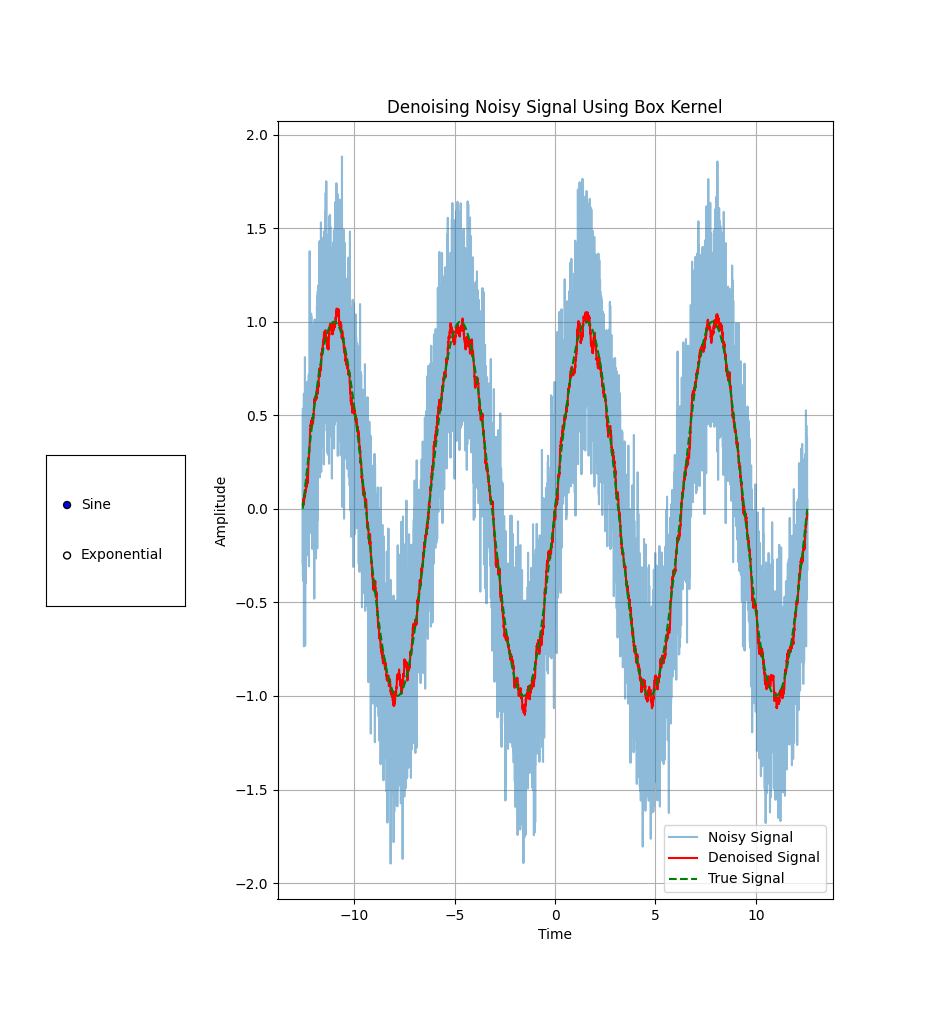
\includegraphics[width = 230pt]{figs/sine_denoise.png}
	\end{subfigure}
	\hspace{110pt}
	\begin{subfigure}[b]{100pt}
		\caption{Exponential}
		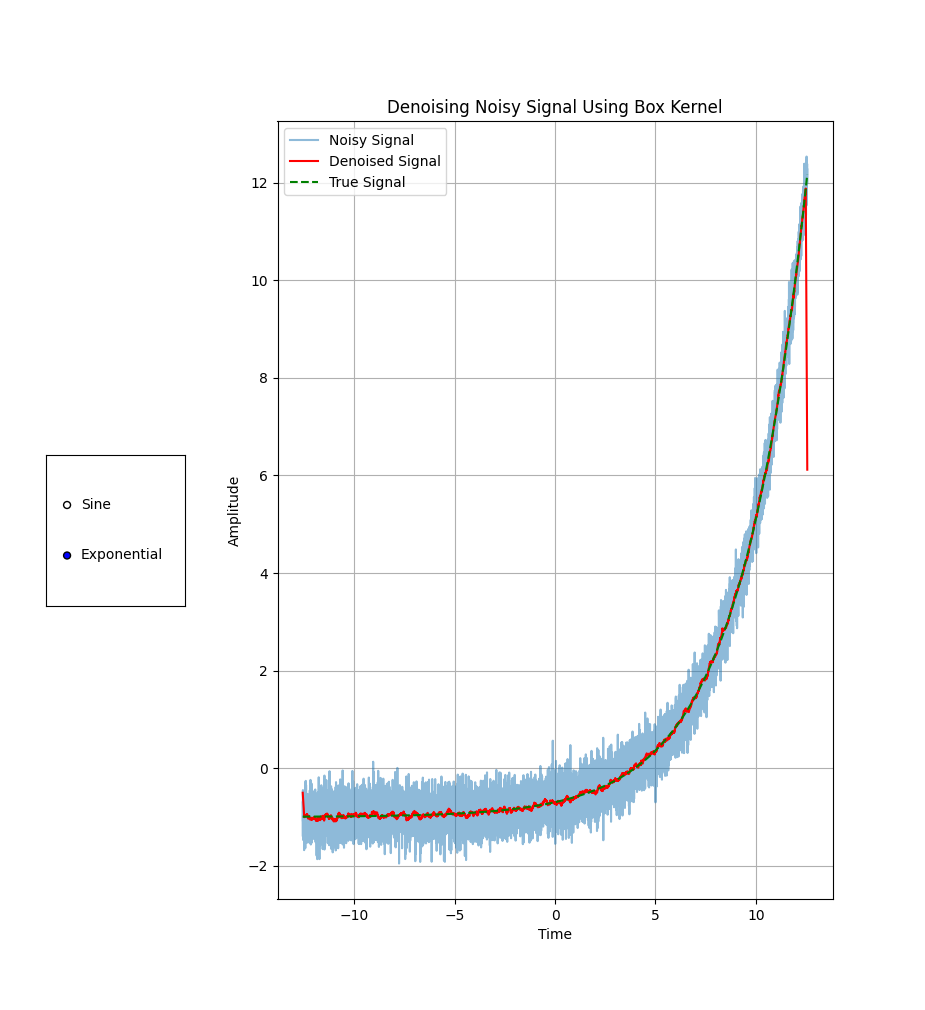
\includegraphics[width = 230pt]{figs/exp_denoise.png}
	\end{subfigure}
\end{figure}

\chapter{Conclusion}

The convolution of various input signals with a rectangular (box) kernel demonstrates how this operation acts as a fundamental smoothing and averaging tool in signal processing. For step, polynomial, sinusoidal, impulse, and exponential inputs, the rectangular kernel produces characteristic effects: smoothing sharp transitions, attenuating high-frequency components, and scaling or shifting the output depending on the kernel width and position. \newline
Adjusting the kernel width 'T' controls the degree of smoothing and detail retention, while time-shifting the kernel introduces corresponding delays in the output. Overall, convolution with a box kernel provides a versatile method for analyzing and processing signals, balancing noise reduction with preservation of essential signal features.
\chapter{Bibliography}
\begin{itemize}
    \item \url{https://www.youtube.com/watch?v=KuXjwB4LzSA}
    \item \url{https://www.youtube.com/watch?v=IaSGqQa5O-M&t=1294s}
    \item \url{https://en.wikipedia.org/wiki/Kernel_(image_processing)}
    \item \url{https://www.geeksforgeeks.org/types-of-convolution-kernels/}
\end{itemize}
\end{document}
